\gls{igro} is an \gls{html} \gls{gui} for the analysis and the integration of multiple \gls{ngs} data with the aid of several already published packages designed for this aim. 

For the \gls{gui} implementation we used the \textit{Shiny} R libraries enabling to render R code in \gls{html} format.

\textbf{ GENERAL DESCRIPTION OF THE INTERFACE }

The tool presents itself with a main upper menu of main topics organized by scope. For each of this topic, a sub-menu with specific functionalities is available.
Moreover, depending on the selected functionality, a side menu is presented with additional functionalities or with input parameter to setup.


\begin{figure}[H]
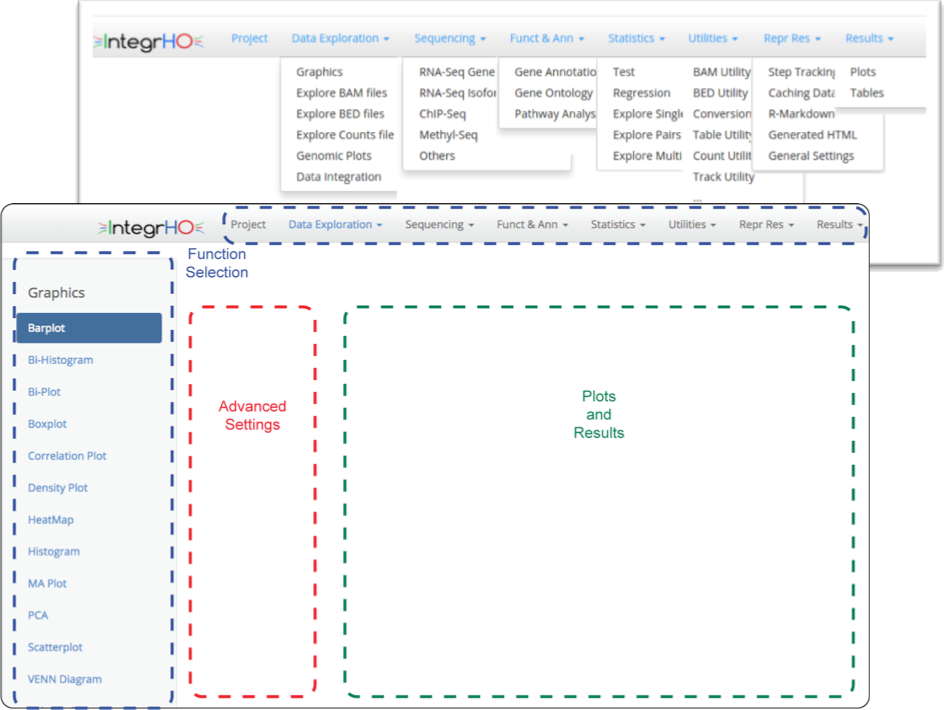
\includegraphics[width=\textwidth,height=\textheight,keepaspectratio]{img/integrho/general_description.png}
\caption[integrho main interface]{}
\label{fig:integrhomain}
\centering
\end{figure}
 

After the parameter setup the results in graphical or table format are presented in the main part of the interface. (figure \ref{fig:integrhomain})


